\documentclass[10pt]{article}
\usepackage[utf8]{inputenc}
\usepackage[swedish]{babel}

\def\poltitle{Sektionens medaljer och dess utdelning}
\def\antagen{2013-11-12}
\def\uppdaterad{2016-11-22}

\usepackage{./e-policy}
\usepackage{../e-styrdok}
\usepackage{../../e-sek}

\begin{document}
\section*{\doctitle}


\subsection*{E-sektionens Funktionärsmedaljer}
Sigillbevararen tillsammans med styrelsen avgör vem som gjort sig förtjänt av en funktionärsmedalj. Detta beslut baseras på om personen i fråga fullgjort sitt åtagande i enlighet med reglementet.

\subsubsection*{Funktionärsmedalj 1 år}
En medalj som tilldelas medlemmar som har varit aktiva inom E-sektionen under ett år och utfört sitt funktionärsåtagande.

\subsubsection*{Funktionärsmedalj 3 år}
Ett tillägg på funktionärsmedaljen som tilldelas medlemmar som har varit aktiva inom E-sektionen under tre år och utfört sina funktionärsåtaganden.

\subsubsection*{Funktionärsmedalj 5 år}
Ett tillägg på funktionärsmedaljen som tilldelas medlemmar som har varit aktiva inom E-sektionen under fem år och utfört sina funktionärsåtaganden.

\subsubsection*{Styrelsemedalj}
Till funktionär som har varit styrelseledamot på E-sektionen.

\subsection*{E-sektionens förtjänstmedaljer}
Mottagare av följande medaljer utses av Sigillbevararen tillsammans med styrelsen. Medaljerna ska utdelas på någon av Sektionens högtidligaste sammankomster som till exempel Nollegasquen eller vid Jubileum dit mottagaren av Krusidull-E:t ska bli inbjuden

\subsubsection*{E-sektionens Bidragsmedalj}
Till medlem av sektionen som har bidragit med något till E-sektionen. Medaljen ges till personer som har lagt ner tid för att förbättra eller ge tillbaka något till E-sektionen. Får utdelas till maximalt tre personer per år.

\subsubsection*{E-sektionens Utomstående Förtjänstmedalj}
Medaljen tilldelas individer som ej är sektionsmedlem och som har bidragit något utöver det vanliga.

\subsubsection*{Krusidull-E}
E-sektionens finaste hedersmedalj tilldelas de E-sektionsmedlemar som utöver det vanliga bidragit med utmärkta insatser för E-sektionen. Utdelandet av Krusidull-E ska vara ytterst restriktivt. De personer som utnämns till hedersmedelmar enligt §2.3.2 i stadgarna ska tilldelas Krusidull-E.

\begin{figure}[H]
\begin{center}
    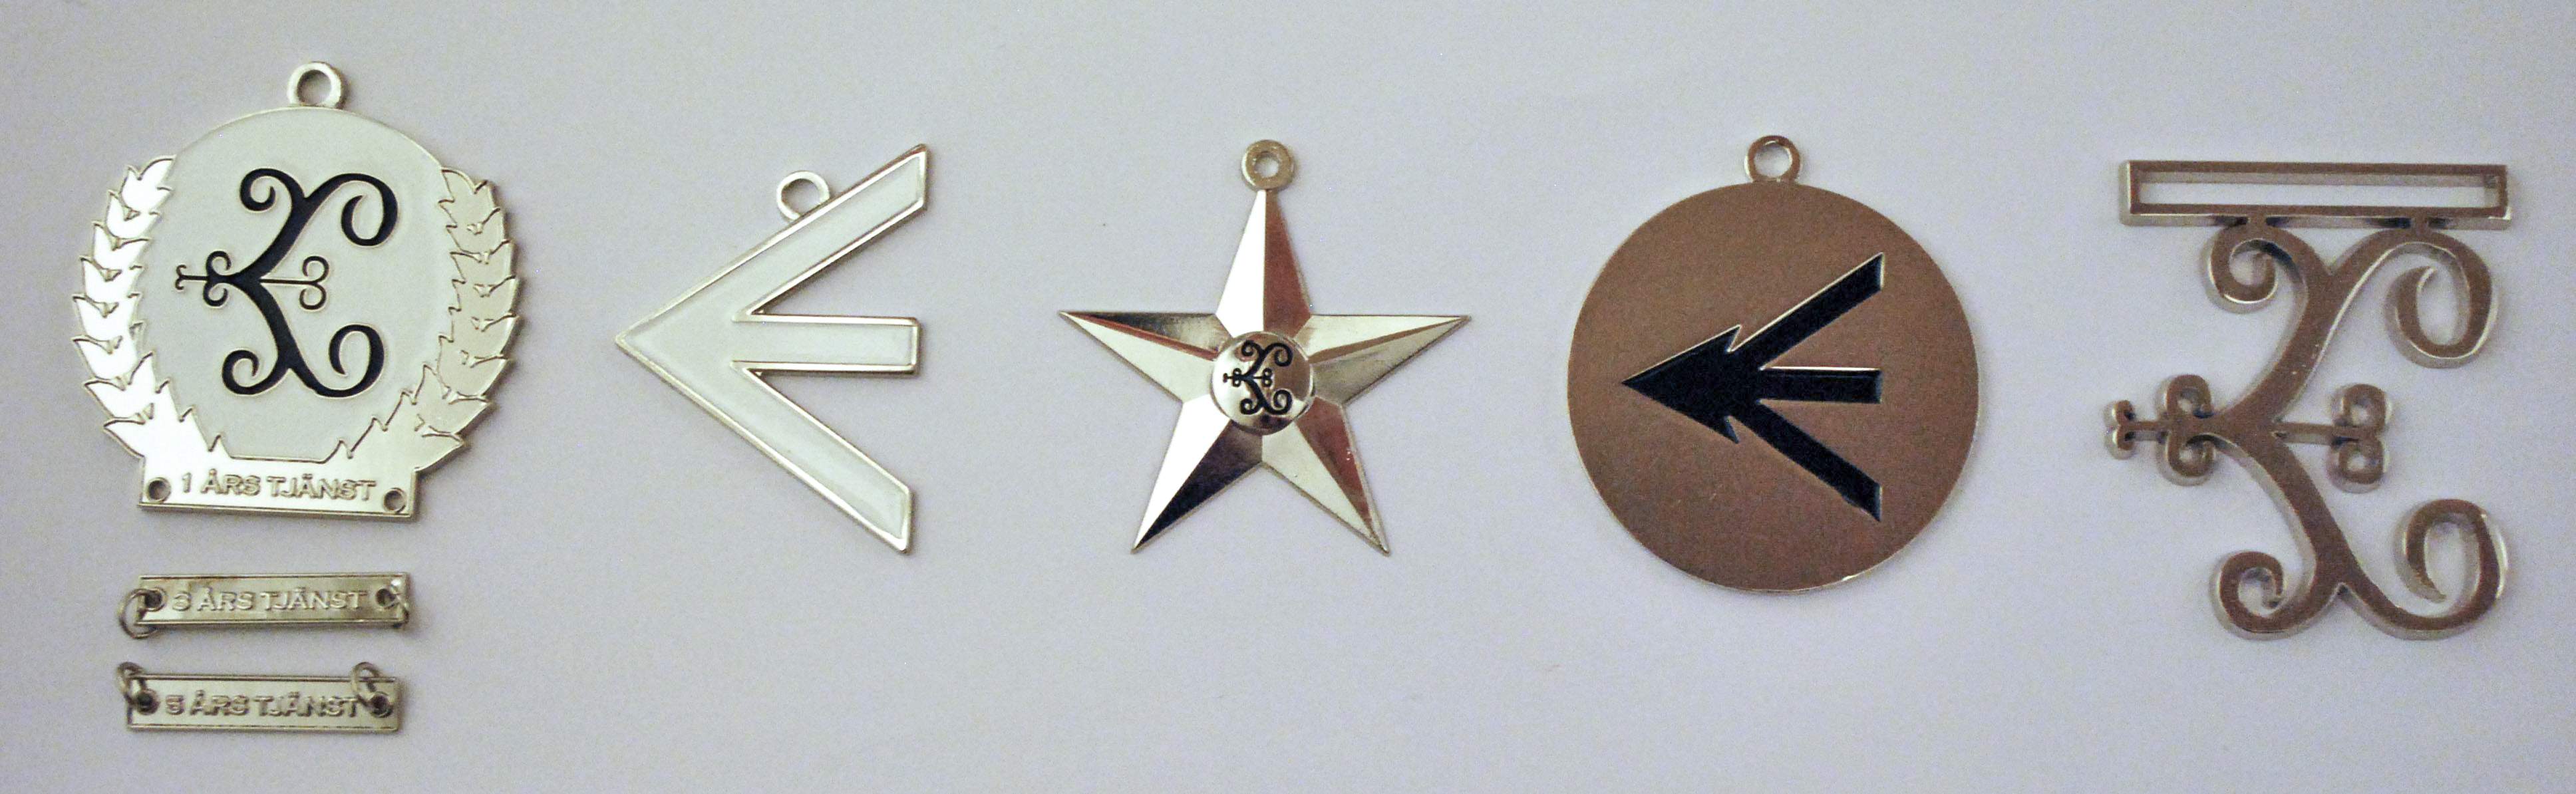
\includegraphics[width=0.9\textwidth]{medaljer.jpg}\\
\end{center}
{Sektionens medaljer. Från vänster: Funktionärsmedalj 1 år med tillägg för 3 samt 5 år, Styrelsemedalj, Bidragsmedalj, Utomstående Förtjänstmedalj samt Krusidull-E.}
\end{figure}

\end{document}
